%\section{Background}
%%Hammond / Srinivas -- you may change the following if you think of a better structure

\ignore{
\subsubsection{\acf{RV}}
Run-time verification is an extension of run-time monitoring~\cite{runtime-verify}.
A run-time verifier monitors the I/O events of a system using a specified safety policy.
The verifier provides positive or negative feedback depending on the I/O of the system, providing a verdict for the current state of the automaton.
The run-time verifier has no knowledge of the inner workings of the system, regarding it as a black box.
This makes it ideal for autonomous systems, where the inner workings are often too complex to be verified.

\subsubsection{\acf{RE}}

\acf{RE} is a subset of \ac{RA} that focuses on formal semantics and blocking, delaying, modifying and/or re-ordering of events in a system. 
\ac{RE} can be transformation or reactive.
Transformational \ac{RE} uses the delaying, buffering and reordering of event to enforce a safety policy, while reactive \ac{RE} uses edit functions to edit events and can be bi-directional.
This paper focuses on reactive \ac{RE}, since \acp{ANN} are reactive in nature.

Processes that are deemed unsafe can be monitored by an enforcer at runtime to ensure that they obey desired policies and remain in a safe state at all times~\cite{theoryRE}. 
Formal runtime verification methodologies mathematically guarantee the detection of improper system behaviour \cite{RuntimeAssuranceForComplexCPS}.
For example, \ac{SA} have been proposed, which formally monitor uni-directional run-time properties only (e.g. outputs only)~\cite{enfsafepol}.
Edit automata are a type of \ac{SA} that can edit, suppress or insert events~\cite{editautomata}. 
\ac{DTA} have been proposed that can edit \textit{bi-directional} events at runtime~\cite{recps}. 
They were designed for reactive \ac{CPS} demonstrated in a pacemaker environment~\cite{recps}. 
Figure~\ref{fig:rebasic} shows the structure of a basic bi-directional run-time enforcer over controller inputs $\{A,B\}$ and controller ouptuts $\{C,D\}$.

\begin{figure}[!htb]
	\centering
	\includegraphics[scale=1.5]{Content/fig/enforced-snns.pdf}
	\caption{Generalised bi-directional enforcer.}
	\label{fig:rebasic}
\end{figure}
}

\section{Motivating Example}
\label{sec:av-casestudy}
%Here we present the overview of the proposed approach that combines SNNs with RE i.e. \acfp{ENN}.
%We also present the case study.

%\subsection{Case Study: \acf{AV}}
%\label{sec:av-casestudy}
\acfp{AV} are \acf{CPS} that are safety critical as highlighted by
recent fatalities involving Tesla and Uber \acp{AV}~\cite{coldewey_2018}~\cite{stewart_2018}.
In this paper, we take inspiration from such accidents and create a case study involving the braking mechanism of \acp{AV}.

\begin{figure}[h]
	\centering
	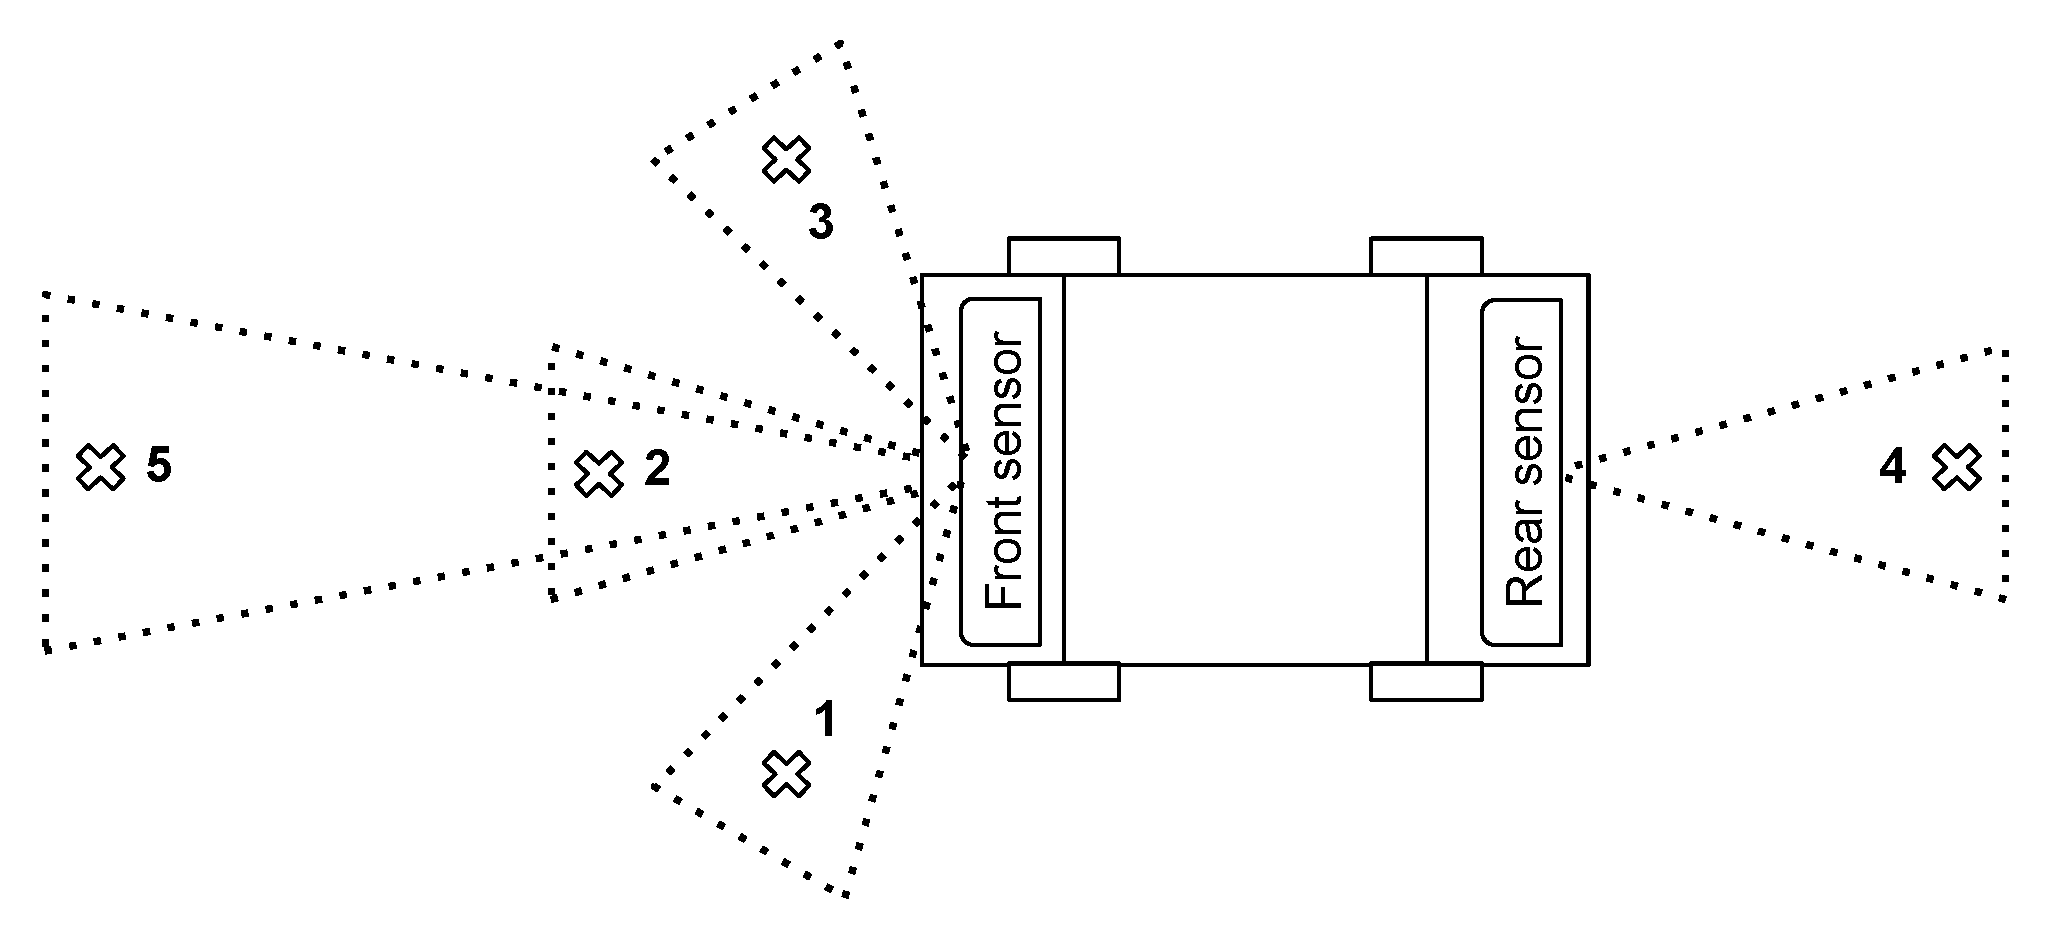
\includegraphics[scale=0.24,trim={0 7mm 0 7mm},clip ]{Content/fig/AV.pdf}
	\caption{Sensor layout for the \ac{AV} example. \label{fig:av}}
\end{figure}
\vspace{1em}
The abstracted \acf{AV} is represented in Figure~\ref{fig:av} .
It will manage forward linear movement of the \ac{AV} and the braking involved with such movement.
The simulation environment consists of one \ac{AV} interacting with other vehicles and pedestrians in its proximity.
The \ac{AV} is run by an autonomous controller with 5 directional sensor inputs, each of which is a camera with its own field of view.
Each camera also features a \acf{LiDAR} sensor for detecting the
distance and shapes of objects in its vicinity.
Each of the five cameras feeds into a \acf{MNN} ensemble~\cite{Maqsood2004} of \acp{SNN}, using the Darknet library~\cite{darknet13}, while the \ac{LiDAR} readings are passed directly to the controller.
\begin{figure}[b]
	\centering
	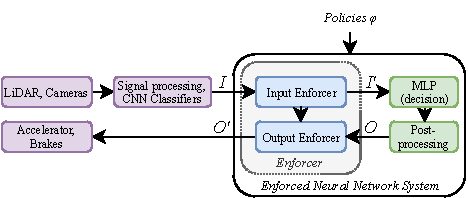
\includegraphics[width = \textwidth]{Content/fig/model-driven-ai-av-example.pdf}
	\caption{Block diagram of \ac{ENN} system used in \ac{AV} case study. \label{fig:avnenf}}
	\vspace{-4mm}
\end{figure}

An \ac{ANN} ensemble is created by execution of multiple \acp{ANN} working in tandem to produce more accurate output~\cite{Maqsood2004}.
%An ensemble can contain different \acp{ANN}, with different structures, inputs, outputs and even programming languages.
%The output of an \ac{ANN} ensemble represents some combination of all the \acp{ANN} in the ensemble, and is more accurate than any individual \ac{ANN} in the ensemble.
These \ac{SNN} ensembles classify their input image and provide a confidence level for the classified image, before passing this information to the controller.
The controller \ac{SNN} is a \ac{MLP}, and decides the best course of action given the environment and the status of the vehicle. 
\ignore{
The current status of the vehicle is noted by the current speed of the
vehicle ($S$) and the previous speed of the vehicle($S'$) obtained in
the previous \emph{tick}.
The controller then outputs one of three commands to the actuators.
These commands are as follows: accelerate ($A$); brake softly ($B_S$);
and brake hard ($B_H$).~\pr{Now our policy allows progressive braking}
}
A block diagram of the \ac{AV} used in this system is shown in Figure~\ref{fig:avnenf}. 

Figure~\ref{fig:avmnn} is an expanded diagram of the \ac{AV} system, showing the \ac{ANN} layout for this system.
Each \ac{MNN} ensemble is labelled by its corresponding sensor number and shows three \acp{CNN} feeding into a single ensemble function for each \ac{MNN}.
The ensemble outputs are then passed to the controller \ac{SNN} \ac{MLP} via the input run-time enforcer.
The controller's decision is made by its \ac{MLP}, and then passed back to the vehicle via the output enforcer.

\begin{figure}[H]
	\centering
	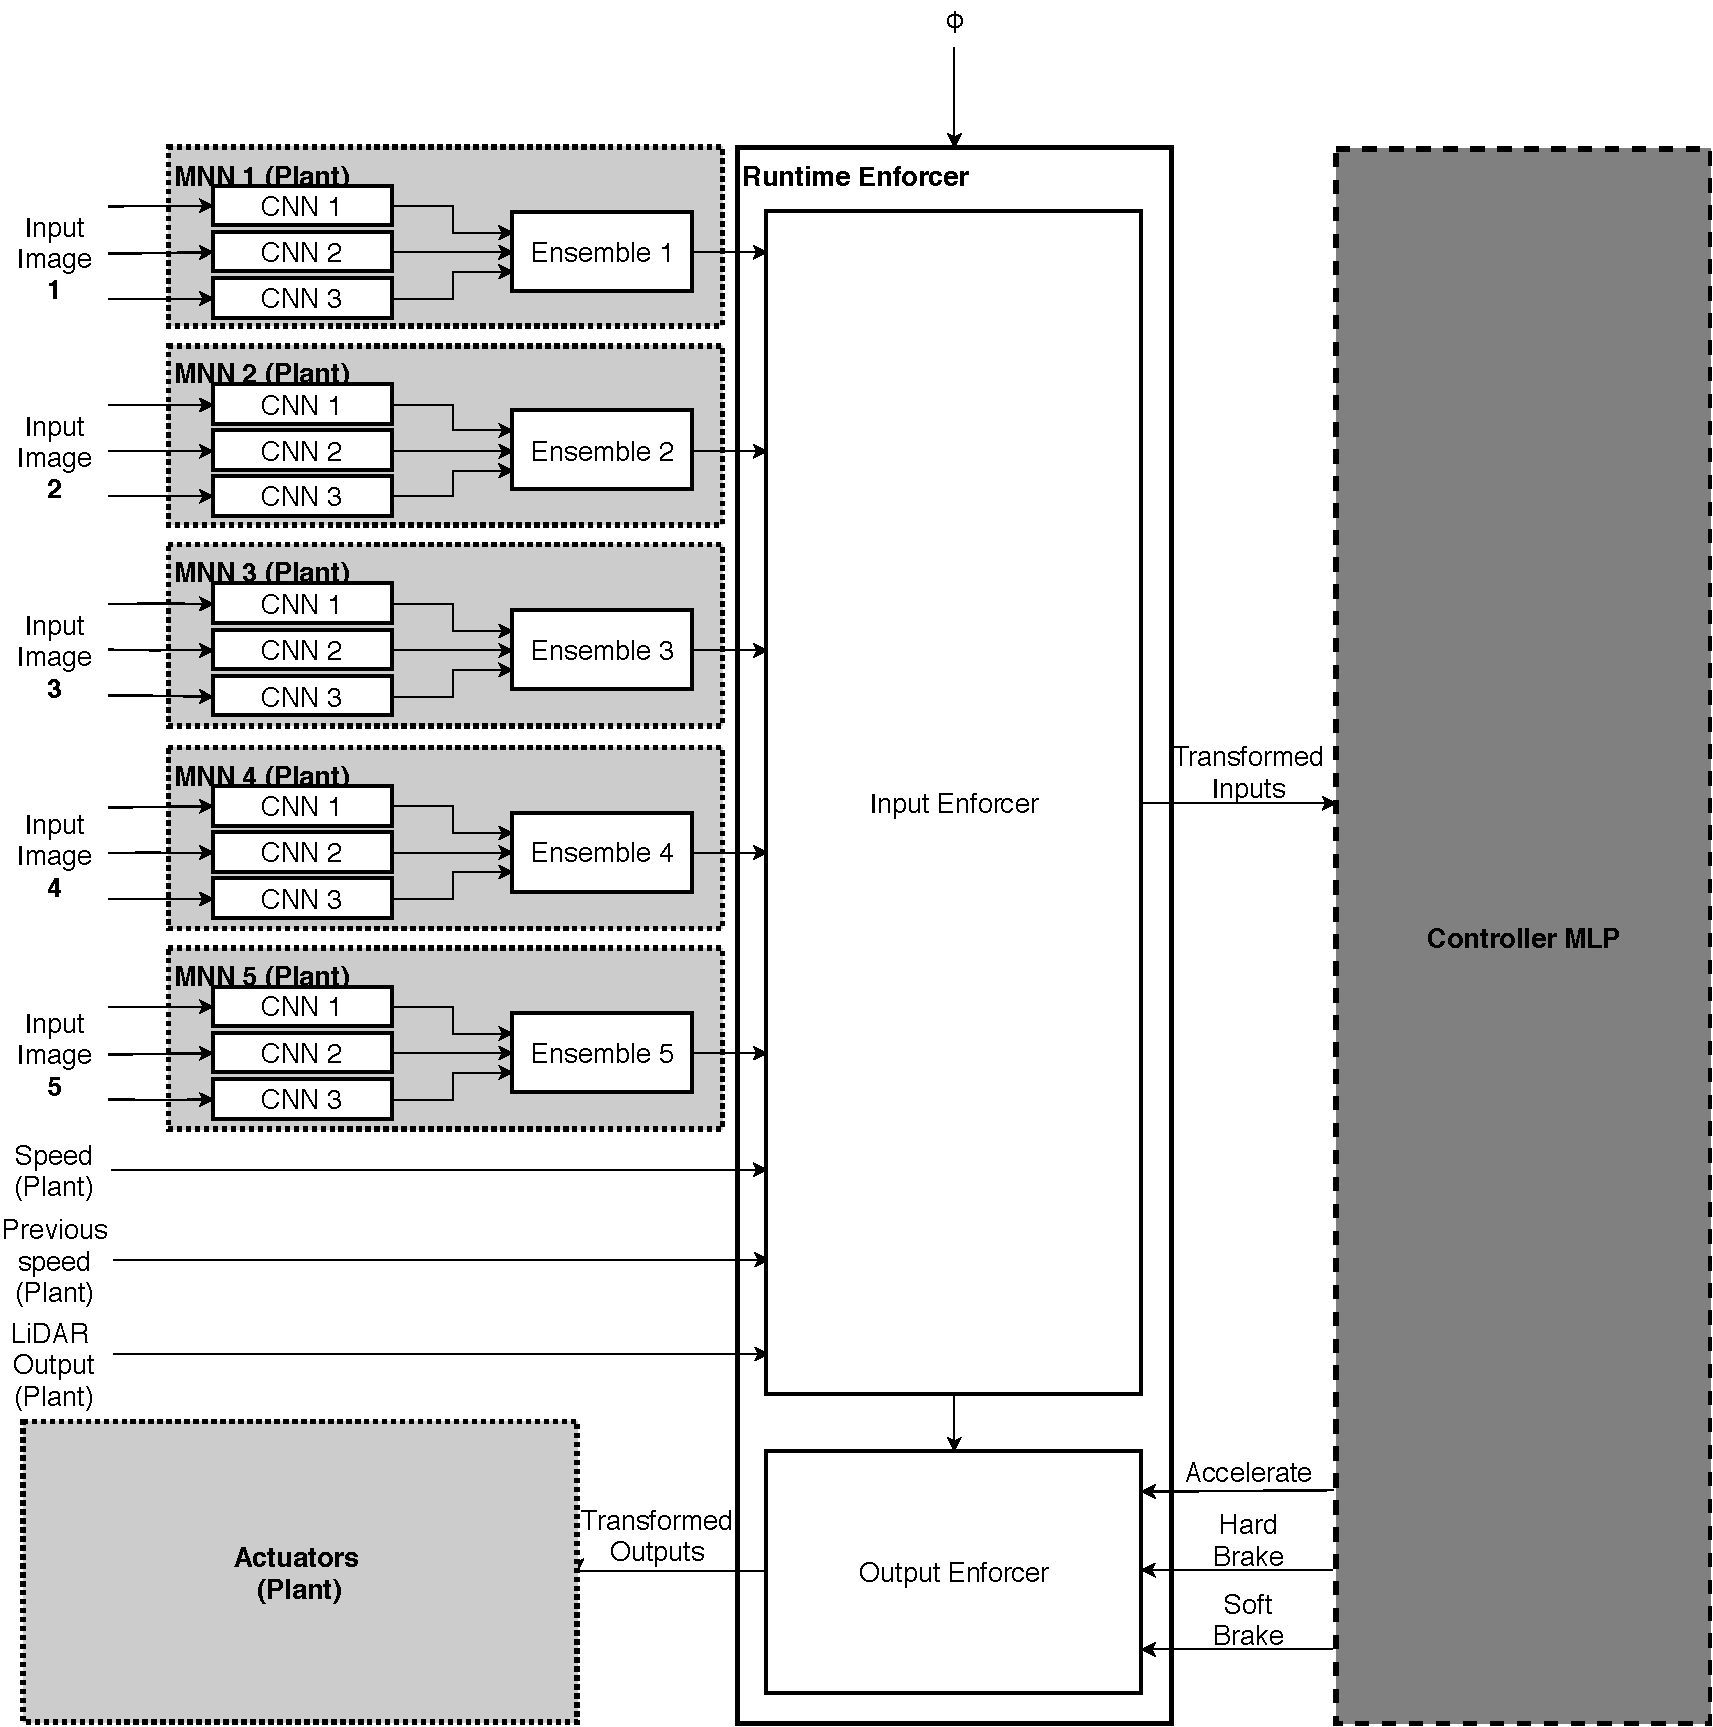
\includegraphics[width=\textwidth]{Content/fig/AV-MNN.pdf}
	\caption{Diagram showing the \ac{SNN} for the \ac{AV}, and its interaction with the plant via the enforcer. \label{fig:avmnn}}
\end{figure}


\ignore{
\subsection{Case Study: \acf{ESS}} \label{sec:ess4}
The \ac{ESS} is inspired by \cite{chaudhari2017hybrid}, in which an \ac{EV} charging station has a separate battery that it uses to assist the charging of the \acp{EV}, with the general idea that the battery is charged when power is cheap, and discharged when demand is high or power is expensive.
The \ac{ESS} uses a pre-trained, three-layer \ac{MLP} to decide the action for the battery in the next tick.
While the \ac{AV} system is a hard real-time system the \ac{ESS} system is a soft real-time system, as a missed deadline will not result in fatalities.
Failures in this system could cause damage to electrical components and potentially cause fires (from overcharging or overcurrent) and maybe even customer property, i.e. the charging station and the \acp{EV}, and thus appropriate policies can be put into place to make the system safer.
\ac{RE} can be used to formally guarantee that the controller will behave safely at all times.
Systems with \acp{ANN} are difficult to verify.
\ac{RE} can ensure that they behave safely even in the event of unexpected inputs.
The enforced policies monitor the controller's \ac{MLP} outputs and ensure that (1) the battery levels never reach critical levels, and (2) that too much power is never given or taken from the battery in too short a period of time.
Running this system with enforced policies shows that the battery's \ac{SoC} never exceeds critical values and that the battery never charges or discharges too much power.
The charge of buying and selling electricity to the customer's \ac{EV} does not change by any significant amount when the enforcer is in place, i.e. it does not affect the performance of the system while it keeps the system safe.}

\section{Valued Discrete Timed Automata}
%In this section, we firstly present some preliminaries and notations
%used. Later we describe the syntax and semantics of the Valued
%Discrete Timed Automata (VDTA).
 We propose \acf{VDTA} to formally represent properties,
 from which enforcement monitors are synthesized. We start with a
 motivating example.

%\todo{This has been lifted from TII and should be rephrased where possible. Examples will be updated of course.}
%\subsection{Preliminaries}
%\todo{SP: added the following paragraph.}
%\red{
%	
%A finite (resp. infinite) word over a finite alphabet $\Sigma$ is a finite sequence $\sigma = a_1\cdot a_2\cdots a_n$ (resp. infinite sequence $\sigma = a_1\cdot a_2\cdots$) of elements of $\Sigma$.
%The set of finite (resp. infinite) words over $\Sigma$ is denoted by $\Sigma^*$ (resp. $\Sigma^\omega$).
%The {\em length} of a finite word $\sigma$ is $n$ and is denoted by $|\sigma|$.
%The empty word over $\Sigma$ is denoted by $\epsilon_\Sigma$, or $\epsilon$ when clear from the context.
%$\Sigma^+$ denotes $\Sigma^*\setminus\{\epsilon\}$.
%The {\em concatenation} of two words $\sigma$ and $\sigma'$ is denoted by $\sigma\cdot \sigma'$.
%A word $\sigma'$ is a {\em prefix} of a word $\sigma$, denoted as $\sigma' \pref \sigma$, whenever there exists a word $\sigma''$ such that $\sigma = \sigma'\cdot \sigma''$; conversely $\sigma$ is said to be an \emph{extension} of $\sigma'$.
%}


\begin{figure}[t]
	\centering
	\scalebox{1}{

\begin{tikzpicture}[>=stealth',shorten >=1pt,auto,node distance=3 cm, scale = 1, transform shape]

\tikzstyle{accept} = [draw=blue!75,fill=blue!20]
\tikzstyle{violate} = [draw=red!75,fill=red!40, dashed]
\tikzstyle{unstable} = [draw=red!75,fill=red!15]

\node[state, initial, accepting, accept] (A) {$l_{safe}$};
\node[state, accepting, accept, unstable] (B) [right of=A] {$l_{brake}$};
\node[state, violate]         (C) [below of=B, yshift=1cm, xshift=-1.5cm]  {$l_v$};

\path[->] 
		(A) edge [loop above,looseness=15]       node [above]  
		{
			\scriptsize$\let\scriptstyle\textstyle\substack{P > 100}$
		} (A)
		
		(A) edge [bend left]		node [above]  
		{
			\scriptsize$\let\scriptstyle\textstyle\substack{P \leq 100, \\ t := 0}$
		} (B)
	
		(B) edge [loop above,looseness=15]		node [above]  
		{
			\scriptsize$\let\scriptstyle\textstyle\substack{\big(P \leq 100~\&~B \geq br\left(P\right)\big)~|\\\big(P > 100~\&~t\leq T_{lim}~\&~B>0\big)}$
		} (B)
	
		(B) edge [bend left]				node [above]  
		{
			\scriptsize$\let\scriptstyle\textstyle\substack{\left(P > 100\right)~\& \\ t > T_{lim}}$
		} (A)
		
		(B) edge [left]			node [right, xshift=0em]  
		{
			\scriptsize$\let\scriptstyle\textstyle\substack{P \leq 100 ~\&~B < br\left(P\right)~|\\
			\big(P > 100~\&~t \leq T_{lim}~\&~B=0\big)}$
		} (C)
	
		(C) edge [loop left]		node [left]  
		{
			\scriptsize$\sum$
		} (C)
		
		;

\end{tikzpicture}}
	\caption{Simplified pedestrian safety policy $\mathcal{A}_{ped}$}
	\label{fig:vdta-car-rte}
\end{figure}

\begin{example}
	\label{eg:vdta}
	%we need values because of tau
	%deadline is a function of the overcurrent value
	
	A pedagogic simplification of pedestrian safety policy is a \ac{VDTA} $\mathcal{A}_{ped}$, as
        depicted in Figure~\ref{fig:vdta-car-rte}.
        The complex policy is used in Section~\ref{sec:resultsc4}.
	%While in reality this is a very complex policy, as the process of detecting a pedestrian relies on processing the data from multiple sensors, we have simplified it in this section for pedagogical purposes.
	%This is a policy involving both valued and timed properties, as follows.
	Assume that we have the input $P$, which represents the distance (in metres) from the car to the nearest pedestrian.
	$P$ is a value from $0$ to $100$ to indicate a valid distance, or $101$ to indicate no pedestrian in range.
	
	In response to a pedestrian at distance $P$, within one tick
        the car should apply brakes by setting the value the actuator
        $B$ as a percentage of maximum braking effort.
	We define function $br: P \rightarrow B$, which takes a
        pedestrian distance $P$ and returns the value of $B$ using $br\left(P\right) = \big(\frac{100 - P}{100}\big)$. 
	Thus, the braking pressure increases linearly based on the distance to the pedestrian. To ensure safety, the car must always apply brakes for a minimum period of time, which we call $T_{lim}$.
	
	%However, due to perturbations in sensory data, the detection methodology for the pedestrian may oscillate around the true value.
	
	%As a result, if a pedestrian is detected, the system should \emph{fail-safe}.
	%To do this, 
	
\end{example}

A VDTA can be seen as an automaton with a finite set of locations, a
finite set of discrete clocks used to represent time evolution, and
external input (resp. output channels) called ``external variables''
which are used for representing system data.They model the data from
the monitored system (resp. environment) read from the input (resp.)
channels in every tick. 
In a \ac{VDTA}, time evolves synchronously: that is, the system executes as a series of discrete \emph{logical ticks} where each tick takes exactly one transition~\cite{SynchronousLanguages12YearsLater}.
In the semantics of VDTA, each transition will be associated with values of external variables.
%They also have internal variables which are used for internal computation, compared to the external variables which model the data carried by the actions from the monitored system (resp. environment). 

\ignore{
Within \ac{VDTA}, there is an implicit logical tick similar to synchronous programming languages
All transitions occur relative to this tick.
At the start of a tick, all input channels are sampled, and at the end of the tick, all output channels are emitted.
Thus, a tick constitutes and atomic reaction of the reactive system.
}

%On transition edges, variables (input and output channels) are updated.
%Static timing analysis techniques can be used to compute .

	
	%	The \ac{VDTA} has a set of actions $\Sigma = \{tk(i, i_{set}, r)\}$.
	%	It consists of only a default ``tick'' action, which represents the ticking of a ``logical clock'' called ``tk''. 
	%	In every tick, the values of all input-output channels are updated.
	
%\end{example}

\subsection{Syntax and Semantics}
We consider our Cyber-Physical Systems to have finite ordered sets of valued input channels ${I} = \{{i_1}, {i_2}, \ldots {i_n}\}$ and valued output channels ${O} = \{{o_1}, {o_2}, \ldots {o_n}\}$.
%Before we look into the formal definition of VDTA, let us consider an example.
%Let us now consider in more detail the syntax and semantics of VDTAs.
%
For a variable (resp. channel) $v$, ${\mathcal D}_v$ denotes its domain,
and for a finite ordered set of variables $V= \{v_1, \ldots, v_n \big\}$,
${\mathcal D}_V$ is the product domain ${\mathcal D}_{v_1} \times \cdots \times {\mathcal D}_{v_n}$.
%A predicate $P(V)$ on a tuple of variables $V$ is a logical formula whose semantics is a function ${\mathcal D}_V \rightarrow \{\true, \false\}$.
A valuation of the variables in $V$
is a mapping $\nu$ which maps every variable $v \in V$ to a value $\nu\big(v\big)$ in ${\mathcal D}_v$.
%
Let $X=\{x_1,\ldots, x_k\}$ be a finite set of integer variables representing discrete clocks.
%
A {\em valuation} for $x$ is an element of $\bbn$, that is a function from $x$ to $\bbn$.
The set of valuations for the set of clocks $X$ is denoted by $\chi$.
%
For $\chi\in\bbn^X$, $\chi+1$ (which captures the ticking of the digital clock) is the valuation assigning $\chi\left(x\right)+1$ to each clock variable $x$ of $X$.
Given a set of clock variables $X' \subseteq X$, $\chi\left[X' \leftarrow 0\right]$ is the valuation of clock variables $\chi$ where all the clock variables in $X'$ are assigned to $0$.


%
\begin{definition}[Syntax of {VDTA}s]
	\label{def:ptav}
	A {VDTA} is a tuple \\
	$\calA = \left(L, {l_0}, X, C, F,  \Delta \right)$ where:
	\squishlist
	%	\item $\Sigma$ is a non-empty finite set of actions,
	%	and an action $a \in \Sigma$ has a signature $sig(a) = ( t_0, t_1, \ldots, t_k )$ which is a tuple of types of the external variables,
	\item $L$ is a finite non-empty set of locations, with $l_0 \in L$ the initial location, and $F \subseteq L$ the set of accepting locations;
	\item $X$ is a finite set of discrete clocks;
	%\item $V$ is a tuple of typed internal variables; 
	\item $C$ is a tuple of external variables, where $C = I \cup O$, where $I$ is the set of input channels, and $O$ is the set of output channels; 
	%\item $\Theta\subseteq {\mathcal D}_{V }$ is an initial condition which is a computable predicate over $V$;
	\item $\Delta$ is a finite set of transitions, and each transition $t \in \Delta$ is a tuple $\left( l, G, A^X, l' \right)$
	also written\\
	$l \xrightarrow{G\left( C \right),A^X} l'$
	such that,
	\squishlist
	\item[\textbullet] $l, l' \in L$ are respectively the origin and target locations of the transition;
	%\item[\textbullet] $c$ is a tuple of external variables;
	\item[\textbullet] $G = G^D \wedge G^X$ is the guard where
	\squishlist
	\item[-] $G^D$ 
	is a computable predicate over external variables  in $C$;
	\item[-] $G^X$ is a clock constraint over $X$ defined as conjunctions of constraints of the form $x \sharp f\left(C\right)$, where $x \in X$ and $f\left(  C \right)$ is a computable function, and $\sharp \in \{ <, \leq, =, \geq, > \}$;
	\squishend
	\item[\textbullet] $A^X \subseteq X$ is the set of clocks to be reset.
	%\item[\textbullet] $A$$=$$(A^D, A^X)$ is the assignment of the transition where
%	\squishlist
	%\item[-] $A^D :{\mathcal D}_V  \rightarrow {\mathcal D}_V$ defines the evolution of internal variables.
	
%	\squishend
	\squishend
	\squishend
\end{definition}
%

\begin{example}	
	
	The \ac{VDTA} for Figure~\ref{fig:vdta-car-rte} has a set of
        locations $L = \{ l_{safe},l_{brake}, l_{v}\}$, with accepting
        locations F = $\{l_{safe}\}$. $l_{safe}$ is also the initial
        location.
	The \ac{VDTA} has the set of external variables  $C = \{P,
        B\}$, where $P$ is an input real-valued channel, 
        and $B$ is an output real-valued channel.
	
	In a VDTA, a transition can have guards on  external variables and clocks. 
	For example, the transition from $l_{safe}$ to $l_{brake}$
        happens when $P \leq 100$. 
	The clock values can be reset upon transitions. 
        For example, upon transition from $l_{safe}$ to $l_{brake}$, the value of clock $t$ is reset to 0.
        
    After a pedestrian is detected, a transition from location $l_{safe}$
    to $l_{brake}$ is taken. 
    Here it must remain as long as two conditions are met.
    Firstly, pedestrian $P$ is within 100 metres.
    Secondly, time $t$ is less than than $T_{lim}$.
    
    There is one violation transition, from $l_{brake}$ to $l_v$. 
    This occurs when either the brakes are not pressed hard enough while the
    pedestrian is within collision range, or if the pedestrian was detected less than $T_{lim}$ time units ago yet the controller has already stopped braking.
\end{example}
%A word is a sequence $\sigma = \eta_1\cdot \eta_2 \cdots \eta_n$ where $\forall i \in [1,n]:$ $\eta_i$ is a tuple of values of variables in $C = I \cup O$.
	
A finite (resp. infinite) word over $\calD_C$ (where $C = I \cup O$) is a finite sequence $\sigma = \eta_1\cdot \eta_2 \cdots \eta_n$ where $\forall t \in [1,n]:$ $\eta_t$ is a tuple of values of variables in $C = I \cup O$. For convenience where necessary, each element $\eta_i$ is considered to be a pair $\left(\eta_I, \eta_O\right)$, where $x_i$ is a valuation of all the variables in $I$, and   $y_i$ is a valuation of all the variables in $O$.
The set of finite (resp. infinite) words over $\calD_C$ is denoted by $\calD_C^*$ (resp. $\calD_C^\omega$).
The {\em length} of a finite word $\sigma$ is $n$ and is denoted by $|\sigma|$.
The empty word over $\calD_C$ is denoted by $\epsilon_C$, or $\epsilon$ when clear from the context.
$\calD_C^+$ denotes $\calD_C^*\setminus\{\epsilon\}$.
The {\em concatenation} of two words $\sigma$ and $\sigma'$ is denoted by $\sigma\cdot \sigma'$.
A word $\sigma'$ is a {\em prefix} of a word $\sigma$, denoted as $\sigma' \pref \sigma$, whenever there exists a word $\sigma''$ such that $\sigma = \sigma'\cdot \sigma''$; conversely $\sigma$ is said to be an \emph{extension} of $\sigma'$.

A property $\varphi$ over $C$ defines a set $\calL\left(\varphi\right)\subseteq \calD_C^{*}$.
A program $\calP \models \varphi$ iff $\calL\left(\calP\right) \subseteq  \calL\left(\varphi\right)$.
In this paper, properties are formally defined as VDTA.

%Policy \ac{VDTA} are required to be \textit{deterministic}, i.e. for any given state, the conjunction of any guards of any other outgoing transitions may not be satisfiable; and \textit{complete}, i.e. for any given state at any given time and any valuation of variables in $C$, at least one transition guard is satisfied.

\subsubsection{Semantics for \ac{VDTA}}

Let $\calA = \left(\Sigma, L, {l_0}, X, C, F,  \Delta \right)$  be a VDTA.
The semantics of $\calA$ is a timed transition system,
where a state consists of a location, and valuations of clocks $X$.
Each transition is associated with values of external variables in $C$.

\begin{definition}[Semantics of {VDTA}s]
	\label{def:vdta:semantics}
	The semantics of $\calA$ is a timed transition system $\sem{\calA}=\left( Q, q_0, Q_F, \Gamma, \to \right)$, defined as follows:
	\squishlist
	\item $Q = L \times \bbn^X$, is the set of states of the form $q= \left( l,\chi \right)$ where
	$l \in L$ is a location,
%	$\nu \in {\mathcal D}_V$ is a valuation of internal variables,
	$\chi$ is a valuation of clocks;
	\item $Q_0 = \{ \left( l_0, \chi_{\left[X \leftarrow 0\right]} \right) \}$ is the set of initial states;
	\item $Q_F = F \times  \bbn^X$ is the set of accepting states;
	\item $\Gamma = \{ \eta \mid
	\eta \in {\mathcal D}_{C}  \}$ is the set of transition labels;
	\item $\to\subseteq Q\times \Gamma\times Q$  the transition relation
	is the smallest set of transitions of the form
	$\left( l,\chi \rangle \longrightarrow {\eta} \langle l',\chi'\right)$
	such that  $\exists \left( l, G, A^X, l' \right) \in \Delta$,
	with $G^X\left(\chi + 1\right) \wedge G^D\left(\eta\right) $ evaluating to {\true},
	%$\nu'= A^D\left(\nu\right)$ 
	and $\chi'=\left(\chi+1\right)[A^X \leftarrow 0]$.
	\squishend
\end{definition}

A {\em run} $\rho$ of $\sem{\calA}$ from a state $q\in Q$ over a {\em trace} $w =  \eta_1\cdot \eta_2\cdots \eta_n$ is a sequence of moves in $\sem{\calA}$:
$\rho = q \xrightarrow {\eta_1} q_1
\cdots q_{n-1}\xrightarrow {\eta_n} q_{n}$,
for some $n\in\bbn$.
A run is accepted if it starts from the initial state $q_0\in Q$ and ends in an accepted state $q_n \in Q_F$.
%The set of runs from the initial state $q_0\in Q$,  is denoted $\Run(\calA)$ and $\Run_{Q_F}(\calA)$ denotes the subset of those runs {\em accepted} by $\calA$, i.e.,  ending in an accepting state $q_n \in Q_F$.

%%%%%%%%%%%%%%%%%%%%%%%%%%%%%%%%%%%%%%%%%%%%%%%
%%%%%%%%%%%%%%%%%%%%%%%%%%%%%%%%%%%%%%%%%%%%%%%
\begin{example}[Run of a VDTA]
	%Let us consider the VDTA %discussed in Example~\ref{eg:vdta}
	%presented in Figure~\ref{fig:vsa-overcurrent}. 
	An example run of the VDTA depicted in Figure~\ref{fig:vdta-car-rte} is elaborated here.
	Assume $T_{lim} = 5$.
	A run of this VDTA starting from the initial state $\left(l_{safe}, t = 0\right)$ for the word $\sigma = \left(101,0\right)\cdot \left(100,0\right)\cdot \left(90,0.2\right)\cdot \left(101,0.2\right)\cdot\left(75,0.4\right)\cdot \left(70,0\right)$ is:\\
	{\small$
		\left(l_{safe}, t = 0\right)
		\xrightarrow {\left(101, 0\right)} 
		\left(l_{safe}, t = 1\right)
		\xrightarrow {\left(100, 0\right)} 
		\left(l_{brake}, t = 0\right)
		\xrightarrow {\left(90, 0.2\right)} \\
		\left(l_{brake}, t = 1\right)
		\xrightarrow {\left(101, 0.2\right)} 
		\left(l_{brake}, t = 2\right)
		\xrightarrow {\left(75, 0.4\right)} 
		\left(l_{brake}, t = 3\right)
		\xrightarrow {\left(70, 0\right)} 
		\left(l_{vio}, t = 4\right).
		$
	}
	
	The run started in the initial state.
	A pedestrian is detected in the second tick, and in the third tick, the \ac{AV} starts braking with $B = 0.2$. 
	This meets the safe threshold.
	In the fourth tick, the input sensor package misclassifies and says that no pedestrian is detected, setting $P = 101$.
	However, the controller continues to brake with $B = 0.2$.
	The pedestrian is re-detected in the fifth tick and the car continues to brake.
	However, in the sixth tick, the controller malfunctions, and even though a pedestrian is still detected, it stops braking.
	As a result, the \ac{VDTA} will go to the non-accepting state $l_v$. 
	This is thus a non-accepting run and represents a violation scenario.
\end{example}
%%%%%%%%%%%%%%%%%%%%%%%%%%%%%%%%%%%%%%%%%%%%%%%%%%%%%%%%%%
\begin{definition}[Deterministic (complete) \ac{VDTA}]
	\label{def:detComplete}
	A VDTA $\calA= \left(L, {l_0}, X, C, F,  \Delta \right)$ with its semantics $\sem{\calA}$ is said to be a {\em deterministic} \ac{VDTA} whenever for any location $l$
	and any two distinct transitions $\left(l,g_1,A^X_1,l'_1\right) \in \Delta$ and $\left(l, g_2, A^X_2, l'_2 \right)\in \Delta$ with same source $l$, the conjunction of guards $g_1\wedge g_2$ is unsatisfiable.
	$\calA$ is {\em complete} whenever for any location $l\in L$ the disjunction of the guards of the transitions leaving $l$ evaluates to {\em true}.
\end{definition}

%%%%%%%%%%%%%%%%%%%%%%%%%%%%%%%%%%%%
\ignore{
\begin{definition}[Product of VDTAs]
	\label{VDTA:product}
	Given two VDTAs 
		\[\calA^{1} = \left(L^{1}, {l_0}^{1}, X^{1}, V^{1}, C^{1}, \Theta^{1}, F^{1},  \Delta^{1} \right)\] and
		\[\calA^{2} = \left(L^{2}, {l_0}^{2}, X^{2}, V^{2}, C^{2}, \Theta^{2}, F^{2},  \Delta^{2} \right)\]
		with disjoint sets of integer clocks (X), internal variables (V) and external variables (C), their product is the VDTA \[\calA^{1}\times \calA^{2}= \left(L, {l_0}, X, V, C, \Theta, F,  \Delta \right)\] where
	$L=L^1 \times  L^2$, $l_0 = (l^1_{0}, l^2_{0})$,  $X  = X^1 \cup X^2$  , $V  = V^1 \cup V^2$ ,  $C  = C^1 \cup C^2$, $F = F^1 \times F^2$, 
 $\Theta = \Theta^{1} \wedge \Theta^{2}$
	and  $\Delta$ 
	is a finite set of transitions where each transition $t=\left( \left(l^{1},l^{2}\right), G^{1}\wedge G^{2}, A^{1} \cup A^{2}, \left(l^{'1},l^{'2}\right) \right)$ belongs to $\Delta$ if $\left( l^{1}, G^{1}, A^{1},l^{'1} \right)$ belongs to $\Delta^{1}$ and  $\left(l^{2}, G^{2}, A^{2},l^{'2} \right)$ belongs to $\Delta^{2}$.
\end{definition}

The product of \acp{VDTA} is useful when we have multiple properties to enforce.
}
%Given two  deterministic and complete \acp{DTA} $\calA^1$ and $\calA^2$ the \ac{DTA} $\calA$ obtained by computing their product recognizes the language $\calL(\calA^1) \cap \calL(\calA^2)$, and is also deterministic and complete.
%%%%%%%%%%%%%%%%%%%%%%%%%%%%%

\subsection{Edit Functions}
\label{sec:editfunc}
The proposed enforcement mechanism is allowed to edit input (resp. output) channels when necessary.
The edit functions that we introduce here will be used in defining the enforcer and  enforcement algorithm in the later sections. 
%%%%%%%%%%%%%%%%%%%%%%%%%%%%

In this framework it is possible to express bi-directional enforcement policies, where
the enforcer has to first transform inputs from the environment in each step according to property $\varphi$ defined as DTA $\calA_\varphi$.
We thus need to consider the input property that we obtain from $\calA_\varphi$ by projecting on inputs.

\begin{remark}[Input \ac{VDTA} $\calA_{I}$]
	\label{def:inp:prop:proj:def}
	Given a property defined as \ac{VDTA} $\calA=\left(L, {l_0}, X, C,  F,  \Delta \right)$, input \ac{VDTA} $\calA_{I}=\left(L, {l_0}, X,  C,  F,  \Delta_I \right)$ is obtained from $\calA$ by ignoring outputs channels on the transitions. For every transition $t \in \Delta$ there will be a transition $t' \in \Delta_I$ where $t' = \left( l, G', A'^X, l' \right)$ is obtained from t = $\left( l, G, A^X, l' \right)$ by discarding all the atomic formulas in $G^{D}$ and $G^{X}$ (which are both Boolean combination of formulas) that has output channels.
	\end{remark}
%
%\begin{definition}[Input \ac{VDTA} $\calA_{I}$]
%	\label{def:inp:prop:proj:def}
%	Given a property defined as \ac{VDTA} $\calA=\left(L, {l_0}, X, C,  F,  \Delta \right)$, input \ac{VDTA} $\calA_{I}=\left(L, {l_0}, X,  C,  F,  \Delta_I \right)$ is obtained from $\calA$ by ignoring outputs channels on the transitions. For every transition $t \in \Delta$ there will be a transition $t' \in \Delta_I$ where $t' = \left( l, G', A', l' \right)$ is obtained from t = $\left( l, G, A, l' \right)$ as follows:
%	\begin{itemize}
%		\item $G' = G^{D'} \wedge G^{X'}$, where  $G^{D'}$ and  $G^{X'}$ are obtained from $G^{D}$ (resp. $G^{X}$) by discarding any disjunct that has an output channel.  
%	\end{itemize}
%\end{definition}




In every tick, the enforcer has to first observe all the input channel values (and edit them if necessary), before it can observe and validate the values of the output channels.  
Input VDTA $\calA_I$  described in remark \ref{def:inp:prop:proj:def} is a property of inputs (only) that we obtain from a VDTA $\calA$ that expresses a property over both inputs and outputs. 
Input \ac{VDTA} may be non-deterministic.


\begin{figure}[tb]
	\centering
	\scalebox{1}{

\begin{tikzpicture}[>=stealth',shorten >=1pt,auto,node distance=3 cm, scale = 1, transform shape]

\tikzstyle{accept} = [draw=blue!75,fill=blue!20]
\tikzstyle{violate} = [draw=red!75,fill=red!40, dashed]
\tikzstyle{unstable} = [draw=red!75,fill=red!15]

\node[state, initial, accepting, accept] (A) {$l_{safe}$};
\node[state, accepting, accept, unstable] (B) [right of=A] {$l_{brake}$};
\node[state, violate]         (C) [below of=B, yshift=1cm, xshift=-1.5cm]  {$l_v$};

\path[->] 
(A) edge [loop above,looseness=15]       node [above]  
{
	\scriptsize$\let\scriptstyle\textstyle\substack{P > 100}$
} (A)

(A) edge [bend left]		node [above]  
{
	\scriptsize$\let\scriptstyle\textstyle\substack{P \leq 100, \\ t := 0}$
} (B)

(B) edge [loop above,looseness=15]		node [above]  
{
	\scriptsize$\let\scriptstyle\textstyle\substack{\big(P \leq 100\big)~|\\\big(P > 100~\&~t\leq T_{lim}\big)}$
} (B)

(B) edge [bend left]				node [above]  
{
	\scriptsize$\let\scriptstyle\textstyle\substack{\left(P > 100\right)~\& \\ t > T_{lim}}$
} (A)

(B) edge [left]			node [right, xshift=0em]  
{
	\scriptsize$\let\scriptstyle\textstyle\substack{P \leq 100~|\\
		\big(P > 100~\&~t \leq T_{lim}\big)}$
} (C)

(C) edge [loop left]		node [left]  
{
	\scriptsize$\sum$
} (C)

;

\end{tikzpicture}}
	\caption{Input VDTA $\mathcal{A}_{ped_I}$ obtained from $\mathcal{A}_{ped}$ in Figure \ref{fig:vdta-car-rte}}
	\label{fig:inp-vdta-car-rte}
	\vspace{-5mm}
\end{figure}

%%%%%%%%%%%%%%%%%%%%%%%%%%%%%
\begin{example}[Input \ac{VDTA} $\calA_{I}$ obtained from $\calA$]
Let us consider the \ac{VDTA} in Figure~\ref{fig:vdta-car-rte} defining the property introduced in Example~\ref{eg:vdta}.
Figure~\ref{fig:inp-vdta-car-rte} presents the input \ac{VDTA} obtained from the \ac{VDTA} in Figure~\ref{fig:vdta-car-rte}.
The violation transition $l_v$ need never be taken, as its guard is also satisfied by the self-loop on $l_{brake}$. 
As a result, $\mathcal{A}_{ped_I}$ will accept all runs, implying $\mathcal{A}_{ped}$ is a uni-directional policy.
\end{example}
%%%%%%%%%%%%%%%%%%%%%%%%%%%%
%%%%%%%%%%%%%%%%%%%%%%%%%%%%%
\paragraph{Edit Functions}
Given property $\varphi\subseteq \calD_C^*$, defined as \ac{VDTA} $\calA_{\varphi}=\left(L, {l_0}, X, C,  F,  \Delta \right)$ with semantics $\sem{\calA_\varphi}=\left( Q, q_0, Q_F, \Gamma, \to \right)$,
%we define and use the following:
we introduce $\editI$ (resp. $\editO$), which the enforcer uses for editing input (resp. output) events (whenever necessary), according to input property $\varphi_I$ (resp. input-output property $\varphi$).
Note that in each step the enforcer first processes the input from the environment, and transforms it using $\editI$ based on the input property $\varphi_I$ obtained from the input-output property $\varphi$ that we want to enforce.
Later, the output produced by the program is transformed by the enforcer (when necessary) using $\editO$ based on the input-output property $\varphi$ that we want to enforce.
%
\squishlist
\item {{\boldmath$\editI\left(\sigma_I\right)$}}:~~Given $I$ (set of input channels), $\editI\left(\sigma_I\right)$ is the set of all possible valuations $\eta_I$ (where $\eta_I$ is a tuple of values of variables in $I$) such that the word obtained by extending $\sigma_I$ with $\eta_I$ can be extended to a sequence that satisfies $\varphi_I$ (i.e., there exists $\sigma'\in \calD_I^*$ such that $\sigma_I\cdot \eta_I \cdot \sigma'$ satisfies $\varphi_I$).
Formally,\\
\[\editI\left(\sigma_I \right) = \{ \eta_I \in \calD_I: \exists \sigma'\in \calD_I^*, \sigma_I \cdot \eta_I \cdot \sigma' \models \varphi_I \}.\]
%Formally, \[\editI(\sigma_I) = \{ x\in \Sigma_I: \sigma_I \cdot x \models \varphi_I \}.\]

Consider the automaton
 $\calA_{\varphi_I}=\left(L, {l_0}, X,  C, F,  \Delta_I \right)$ with semantics $\sem{\calA_{\varphi_I}}=\left( Q, q_{0_I}, Q_{F_I}, \Gamma_I, \to_I \right)$.
 Let $q_I\in Q_I$ correspond to a state reachable in $\calA_{\varphi_I}$ (i.e., $q_{0_I} \xrightarrow{\sigma_I} q_I$) upon $\sigma_I$.
 	We define $\editIaut\left(q_I\right)$ as follows:
\[\editIaut\left( q_I \right) = \{ \eta_I \in \calD_I: \exists \sigma'\in \calD_I^*, q_I \xrightarrow{\eta_I \cdot \sigma'}_I q{'{_I}} \wedge q{'{_I}} \in Q_{F_I} \}.\]

%%%%%%%%%%%%%%%%%%%
%\begin{example}
%\todo{SP: add example..}
%\end{example}
%%%%%%%%%%%%%%%%%%%
\item {\boldmath$\editO\left(\sigma, \eta_I\right)$}:
~~Given an input-output word $\sigma\in \calD_C^*$ and an input event $\eta_I\in \calD_I$, $\editO\left(\sigma, \eta_I\right)$ is the set of valuations of output channels $\eta_O$ in $O$ such that the input-output word obtained by extending $\sigma$ with $(\eta_I,\eta_O)$ can be extended to a sequence that satisfies the property $\varphi$ (i.e., $\exists \sigma' \in \calD_{C}^*$ such that $\sigma\cdot(\eta_I,\eta_O)\cdot\sigma'\models\varphi$).
Formally,
\[\editO\left(\sigma,\eta_I\right) = \{\eta_O \in \calD_O: \exists \sigma'\in \calD_{C}^*, \sigma \cdot \left(\eta_I,\eta_O\right) \cdot \sigma' \models \varphi \}.
\]

%
Consider the \ac{VDTA} $\calA_{\varphi}\left(L, {l_0}, X, C, F,  \Delta \right)$ defining property $\varphi$ with semantics $\sem{\calA_\varphi}=\left( Q, q_{0}, Q_{F}, \Gamma, \to \right)$, and an input event $\eta_I\in \calD_I$.
If $q\in Q$ corresponds to a state reached in $\calA_{\varphi}$ upon $\sigma$ (i.e., $q_{0} \xrightarrow{\sigma} q$), $\editO\left(\sigma, \eta_I\right)$ can be alternatively defined as follows:
%
%
\\
$\editOaut\left(q,\eta_I\right) = \{\eta_O \in \calD_O: \exists \sigma'\in \calD_C^*, q \xrightarrow{\left(\eta_I,\eta_O\right) \cdot \sigma'} q' \wedge q' \in Q_F \}.$

%%%%%%%%%%%%%%%%%%%%%%%%%
\paragraph{Selecting edits}
For any given violation transition (e.g. $q \xrightarrow{\left(\eta_I,\eta_O\right)} q' \wedge q' \notin Q_F$)
there may be many possible alternate values for $\eta_I$ and $\eta_O$ that would instead result in an accepting transition.
To solve this issue, we define two additional functions, $\selEditI$ and $\selEditO$ which the designer can use to \emph{select} a given edit by the designer from the set of possible accepting edits.

\begin{example}
Consider the case in Figure~\ref{fig:vdta-car-rte} where the violation transition to $l_v$ occurs if $P \leq 100~\&~B < br\left(P\right)$.
$\editO$ will suggest as valid edits every value $B \geq br\left(P\right)$, as this would invalidate the violation transition guard.
However, this suggestion is infinite in size for real-valued $B$.
As a result, the designer selects edit $B = br\left(P\right)$, which is a valid edit in the solution space.
\end{example}

%%%%%%%%%%%%%%%%%%%%%%%%%
\item
{\boldmath$\selEditI\left(\sigma_I\right)$:}~~ Given $\sigma_I\in \calD_I^*$ if $\editI\left(\sigma_I\right)$ is non-empty, then $\selEditI\left(\sigma_I\right)$ returns an element (chosen by the designer) from $\editI\left(\sigma_I\right)$, and is undefined if $\editI\left(\sigma_I\right)$ is empty.
Given $q_I\in Q_I$, if $\editIaut\left(q_I\right)$ is non-empty, then $\selEditIaut\left(q_I\right)$ returns an element (chosen by the designer) from $\editIaut\left(q_I\right)$, and is undefined if $\editIaut\left(q_I\right)$ is empty.
\item {\boldmath$\selEditO\left(\sigma,x\right)$:}~~ Given $\sigma\in \calD_{C}^*$, and $x\in \calD_I$,  if $\editO\left(\sigma,x\right)$ is non-empty, then $\selEditO\left(\sigma,x\right)$ returns an element (chosen by the designer) from $\editO\left(\sigma,x\right)$, and is undefined if $\editO\left(\sigma,x\right)$ is empty.
%
Given $q\in Q$ and $x \in \calD_I$, if $\editOaut\left(q,x\right)$ is non-empty, then $\selEditOaut\left(q,x\right)$ returns an element (chosen by the designer) from $\editOaut\left(q,x\right)$, and is undefined if $\editOaut\left(q,x\right)$ is empty.
%


\ignore{

\item {\boldmath$\minEditI\left(\sigma_I, x\right)$:}~~ Given $\sigma_I\in \calD_I^*$ and $x\in \calD_I$, if $\editI\left(\sigma_I\right)$ is non-empty, then $\minEditI\left(\sigma_I, x\right)$ returns an event from $\editI\left(\sigma_I\right)$ with minimal distance\footnote{Distance between two events belonging to the same alphabet is the number of bits that differ in both the events.} w.r.t $x$, and is undefined if $\editI(\sigma_I)$ is empty.
%%%%%%%%%%%%%%%%%%%%%
%
Given $q_I\in Q_I$ and $x \in \calD_I$, if $\editIaut\left(q_I\right)$ is non-empty, then $\minEditIaut\left(q_I, x\right)$ returns an event from $\editIaut\left(q_I\right)$ with minimal distance w.r.t $x$, and is undefined $\editIaut\left(q_I\right)$ is empty.
%%%%%%%%%%%%%%%%%%%%%
\item {\boldmath$\minEditO\left(\sigma, x, y\right)$:}~~ Given $\sigma\in \calD_{C}^*$, $x\in \calD_I$ and $y\in \calD_O$, if $\editO\left(\sigma,x\right)$ is non-empty, then $\minEditO\left(\sigma, x, y\right)$ returns an event from $\editO\left(\sigma,x\right)$ with minimal distance w.r.t $y$, and is undefined if $\editO\left(\sigma, x\right)$ is empty.
%
Given $q\in Q$, $x\in \calD_I$ and $y\in \calD_O$, if $\editOaut\left(q,x\right)$ is non-empty, then $\minEditOaut\left(q, x, y\right)$ returns an event from $\editOaut\left(q,x\right)$ with minimal distance w.r.t $y$, and is undefined $\editOaut\left(q,x\right)$ is empty.
%

}

\squishend
%%%%%%%%%%%%%%%%%%%%%%%%%%%%%%%%%%%%%%%%%%%
%%%%%%%%%%%%%%%%%%%%%%%%%%%%%%%%%%%%%%%%%%%
\section{Enforcer for \ac{VDTA} Properties}
%%%%%%%%%%%%%%%%%%%%%%%%%
An enforcer monitors and corrects both input and output of a system according to a given correctness property $\varphi$.
To synthesise an enforcer for a given property $\varphi$ defined as a \ac{VDTA} $\calA_\varphi$, we borrow from the semantics presented in \cite{RuntimeEnforcementOfCPS}.

An enforcer for a property $\varphi$ can only edit an input-output event when necessary, and it cannot block, delay or suppress events.
Let us recall the two functions $\editI$ and $\editO$ that were introduced in Section~\ref{sec:editfunc} that the enforcer for $\varphi$ uses to edit the current input (respectively output) event according to property $\varphi$.

An enforcer for a given property defined as a VDTA $\calA_\varphi$ can be thought as a function $E_{\calA_\varphi}:{\calD}_{C}^* \rightarrow {\calD}_{C}^*$. 
%These actions represent invocations of our \ac{VDTA}, where the values of input channels $I$ and output channels $O$ may be updated.
The enforcer aims to keep the property $\calA_\varphi$ satisfied, and so will examine the updated external variables (input and output channels) each tick, and will transform any that are non-accepting.

It can be trivial to derive enforcers for a properties which do not behave in a useful manner.
For instance, in the example presented in Figure~\ref{fig:vdta-car-rte}, a trivial enforcer would simply keep the output brakes command $B$ set to 100\% at all times.
This would keep the policy satisfied, but it would not result in a useful \ac{AV}.

To prevent this (and other situations), several constraints are provided which define enforcer correctness~\cite{RuntimeEnforcementOfCPS}.


%%%%%%%%%%%%%%%%%%%%%%%%%%%%%%%%%%%%%%%%%%%%%%
\begin{definition}[Enforcer for $\varphi$]
	\label{def-E-func-constraints}
	Given property $\varphi\subseteq\calD_C^*$, an {\em enforcer} for $\varphi$ is a function $\ef: \calD_C^*\rightarrow \calD_C^*$ satisfying the following constraints:
	%
	
	{\bf Soundness}
	\begin{equation}
	\tag{\bf Snd}\label{eq:snd}
	\forall \sigma \in \calD_C^*, \exists \sigma' \in \calD_C^*:  E_{\varphi}\left(\sigma\right)\cdot \sigma' \models \varphi.
	\end{equation}
	%
	{\bf Monotonicity}
	\begin{equation}
	\tag{\bf Mono}\label{eq:mono}
	\forall \sigma, \sigma' \in \calD_C^*: \sigma\pref \sigma' \Rightarrow \ef\left(\sigma\right) \pref \ef\left(\sigma'\right).
	\end{equation}
	%
	{\bf Instantaneity}
	\begin{equation}
	\tag{\bf Inst}\label{eq:inst}
	\forall \sigma \in \Sigma^*: |\sigma| =  |\ef\left(\sigma\right)|.
	\end{equation}
	%
	{\bf Transparency}
	\begin{equation}
	\tag{\bf Tr}\label{eq:tr}
	\begin{array}{ll}
	\forall \sigma\in \calD_C^*, \forall \eta_I \in \calD_I, \forall \eta_O \in \calD_O, \exists \sigma' \in \calD_C^*:\\
	~~~~~\ef\left(\sigma\right)\cdot\left(\eta_I, \eta_O\right) \cdot \sigma' \models \varphi\\
	~~~~~ \Rightarrow \ef\left(\sigma\cdot\left(\eta_I, \eta_O\right) \right) = \ef\left(\sigma\right)\cdot\left(\eta_I, \eta_O\right) .
	\end{array}
	\end{equation}
	%
	{\bf Causality}
	\begin{equation}
	\tag{\bf Ca}\label{eq:ca}
	\begin{array}{ll}
	\forall \sigma \in \calD_C^*, \forall \eta_I \in \calD_I,\forall \eta_O \in \calD_O,\\
	~~~\exists \eta_I' \in \editI\left(\left(\ef\left(\sigma\right)\right)_I\right), \exists \eta_O' \in \editO\left(\ef\left(\sigma\right), \eta_I'\right):\\
	~~~~~\ef\left(\sigma\cdot\left(\eta_I,\eta_O\right)\right)= \ef\left(\sigma\right)\cdot\left(\eta_I',\eta_O'\right).
	\end{array}
	\end{equation}
\end{definition}
%%%%%%%%%%%%%%%%%%%%%%%%%%%%%%%%%%%%%%%%%%%%%%%%%%%%


\squishlist
\item An enforcer must be \textit{sound}, meaning that for any word $\sigma$ given as input, the output of the enforcer $E_\varphi\left(\sigma \right)$ should satisfy the property $\varphi$.
\item An enforcer must be \textit{transparent}, meaning that the enforcer must edit the actual input and output channel values only when necessary (i.e., only when they lead to violation of the property).
\item An enforcer is \textit{online}, so it cannot undo what is released as output (\textit{monotonicity}), and it must not delay, insert, or suppress ticks (\textit{instantaneity}).
\item An enforcer must be \textit{causal}, meaning that the enforcer must act as an intermediary such
that it first examines values of the input channels to validate them w.r.t property $\varphi$. If the actual input values will lead to a violation, the enforcer may change/correct the inputs before
forwarding to the program. After the program reacts to these inputs, the enforcer must again validate the outputs from the program. It should forward the outputs from the program (without editing) to the environment if they do not lead to a violation, or edit and forward the edited values.  
\squishend
%%%%%%%%%%%%%%%%%%%%%%%%%
%%%%%%%%%%%%%%%%%%%%%%%%%%%%%%%%%%%%
\begin{definition}[Enforceability]
	Let $\varphi\subseteq\calD_C^*$ be a property. We say that $\varphi$ is {\em enforceable} iff an enforcer $\ef$ for $\varphi$ exists according to Definition~\ref{def-E-func-constraints}.
\end{definition}
%%%%%%%%%%%%%%%%%%%%%%%%%%%%%%%%%%%%
%%%%%%%%%%%%%%%%%%%%%%%%%%
%\begin{theorem}[Condition for enforceability]
%	\label{theorem:nonEnf}
%	\todo{SP: to complete}
%\end{theorem}
%%%%%%%%%%%%%%%%%%%%%%%%%%

%%%%%%%%%%%%%%%%%%%%%%%%%	
%Let us recall that an input event $(x,y)$ is a tuple, where $x$ is the input (values of all Boolean inputs), and $y$ is the output (values of all Boolean outputs).
%At each step, the enforcer consumes an input event $(x,y)$ and produces an output event $(x',y')$ by editing $x$ and $y$ if necessary.


%We assume that the controller (pacemaker) may be invoked through a special function call called $\ptick$.
%Since the pacemaker is considered to be a black-box, internals of the function $\ptick$ are considered to be unknown.
%Formally, $\ptick$ is a function (with internal state) from $\Sigma_I$  to  $\Sigma_O$  that takes a bit vector $x \in \Sigma_I$ and returns a bit vector $y \in \Sigma_O$.

%
%At an abstract level, an enforcer may be viewed as a function that transforms words.
%An enforcement function for a given property $\varphi$ takes as input a word over $\Sigma^*$ and outputs a word over $\Sigma^*$ that satisfies $\varphi$, or can be extended to satisfy $\varphi$ in the future.
%

%\paragraph{Soundness}
%(\ref{eq:snd}) means that for any input word $\sigma\in\Sigma^*$, the output of the enforcer $\ef(\sigma)$ can be extended to a sequence that satisfies $\varphi$ (i.e., $\exists \sigma'\in\Sigma^*: \ef(\sigma)\cdot\sigma'\models \varphi$).
%%%
%\paragraph{Monotonicity}
%(\ref{eq:mono}) expresses that the output of the enforcer for an extended input word $\sigma'$ of an input word $\sigma$, extends the output produced by the enforcer for $\sigma$.
%The monotonicity constraint means that the enforcer cannot undo what is already released as output.
%%%
%\paragraph{Instantaneity}
%(\ref{eq:inst}) expresses that for any given input sequence $\sigma$, the output of the enforcer $\ef(\sigma)$ should contain exactly the same number of events that are in $\sigma$ (i.e., $|\sigma| = |\ef(\sigma)|$).
%This means that, the enforcer cannot delay, insert and suppress events.
%Whenever the enforcer receives a new input event, it must react instantaneously and produce an output event immediately.
%This requirement is essential for the enforcement of \acp{CPS}, which are reactive in nature.
%%%
%\paragraph{Transparency}
%Transparency means that the enforcer will not unnecessarily edit any event.
%Any new input event $(x,y)$ will be simply forwarded by the enforcer if what has been computed as output earlier by the enforcer followed by $(x,y)$ can be extended to a sequence that satisfies $\varphi$ in the future.
%
%(\ref{eq:tr}) expresses that for any given input sequence $\sigma$ and any input event $(x,y)$, if the output of the enforcer for $\sigma$ (i.e., $\ef(\sigma)$) followed by the input event $(x,y)$ has an extension $\sigma'\in\Sigma^*$ such that $\ef(\sigma)\cdot(x,y)\cdot\sigma'$ satisfies the property $\varphi$, then the output that the enforcer produces for input $\sigma\cdot(x,y)$ will be $\ef(\sigma)\cdot(x,y)$.
%%%
%\paragraph{Causality}
%(\ref{eq:ca}) expresses that for every input event $(x,y)$ the enforcer produces output event $(x',y')$ where
%the enforcer first processes the input part $x$, to produce the transformed input $x'$ according to property $\varphi$ using $\editI$.
%The enforcer later reads and transforms output $y\in\Sigma_O$ (output of the program after invoking function $\ptick$ with $x'$), to produce the transformed output $y'$ using $\editO$.
%
%The input-output sequence released as output by the enforcer upon reading the input-output sequence $\sigma$ is $\ef(\sigma)$ and $(\ef(\sigma))_I \in \Sigma_I^*$ is the projection on the inputs.
%$\editI(\ef(\sigma))_I)$ returns a set of input events in $\Sigma_I$, such that $\ef(\sigma))_I$ followed by any event in $\editI(\ef(\sigma))_I)$ satisfies $\varphi_I$.
%%Thus, $\editI(\ef(\sigma))_I)$ cannot be empty.
%
%$\editO(\ef(\sigma)), x')$ returns a set of output events in $\Sigma_O$, such that for any event $y$ in $\editO(\ef(\sigma)), x')$, $\ef(\sigma))\cdot(x',y)$ satisfies $\varphi$.
%%%%%%%%%%%%%%%%%%%%%%%%%%%%%%%%%%%%%
%%%%%%%%%%%%%%%%%%%%%%%%%%%%%%%%%%%%%
\section{Runtime Enforcment Algorithm}
\label{sec:re-algorithm}

Let the automaton $\calA_{\varphi}=\left(L, {l_0}, X,  C,  F,  \Delta \right)$ with semantics $\sem{\calA_\varphi}=\left( Q, q_0, Q_F, \Gamma, \to \right)$ define property $\varphi$.
\\ Input automaton $\calA_{\varphi_I}=\left(L, {l_0}, X,  C,  F,  \Delta_I \right)$ with semantics $\sem{\calA_\varphi{_I}}=\left( Q, q_0, Q_F, \Gamma, \to_I \right)$ is obtained from $\calA_{\varphi}$ by projecting on inputs (See section~\ref{sec:editfunc}).

\begin{algorithm}[ht]
	\caption{$\mathsf{Enforcer}$}
	\label{algo:enf}
	{
		\begin{algorithmic}[1]
			\STATE $t \gets 0$
			\STATE $q \gets q_{0}$
			\WHILE {$\true$}
				\STATE $\eta_{It} \gets \readInp\left( \right)$
				\label{algoEi-begin}
				\IF {$\exists \sigma'_I\in\calD_I^*: q \xrightarrow{\eta_{It} \cdot \sigma'_I}_I q' \wedge q' \in Q_{F}$}
					\label{algoEi-test}
					\STATE $\eta'_{It} \gets \eta_{It}$
				\ELSE
					\STATE $\eta'_{It} \gets \selEditIaut\left(q\right)$
				\ENDIF
				\label{algoEi-end}
				\STATE $\mathsf{call\_neural\_network\_\lambda\left(\eta'_{It}\right)}$
				\STATE $\eta'_{Ot} \gets \readOut\left( \right)$
				\label{algoEo-begin}
				\IF {$\exists \sigma'\in\calD_C^*: q\xrightarrow{\left(\eta'_{It},\eta_{Ot}\right)\cdot \sigma'} q' \wedge q' \in Q_F$}
					\label{algoEo-test}
					\STATE $\eta'_{Ot} \gets \eta_{Ot}$
				\ELSE
					\STATE $\eta'_{Ot} \gets \selEditOaut\left(q, \eta'_{It}\right)$
				\ENDIF
				\label{algoEo-end}
				\STATE $\release\left(\left(\eta'_{It}, \eta'_{Ot}\right)\right)$
				\label{algoEo-release}
				\STATE $q \gets q''$ ~~~~ {\footnotesize{where $q\xrightarrow{\left(\eta'_{It},\eta'_{Ot}\right)} q''\wedge q'' \not\in q_v $}}
				\label{algo-stateUpdate}
			%\STATE \red{$q_I \gets q''_I$} ~~~~ {\footnotesize{where $q_I \xrightarrow{x'_t}_I q''_I$}}
				\STATE $t \gets t+1$
			\ENDWHILE
		\end{algorithmic}
	}
\end{algorithm}

We provide an online algorithm that requires automata $\calA_{\varphi}$ and $\calA_{\varphi_I}$ as input.
Algorithm~\ref{algo:enf} is an infinite loop, and an interaction of the algorithm is triggered at every time step.
We join this algorithm to the neural networks through a \emph{reactive interface}, following the structure presented in Figure~\ref{fig:rebasic}.
The \ac{MNN} system thus replaces connections to the enforced \ac{SNN} with connections to the run-time algorithm, and the run-time algorithm passes data to and from the \ac{SNN} by calling the instantaneous network function  $\mathsf{call\_neural\_network\_\lambda\left(\eta'_{It}\right)}$.

In Algorithm~\ref{algo:enf}, $t$ keeps track of the time-step (i.e. \emph{tick}), and is initialized at 0, while $q$ keeps track of the state of both automata $\calA_{\varphi}$ and $\calA_{\varphi_I}$.
Note that $q$ contains information about the current location $l$, the current valuations of internal variables $\nu$, and the current valuations of the clocks $\chi$.
As the automaton $\calA_{\varphi_I}$ is created from $\calA_{\varphi}$ by projecting over the inputs, it therefore has an identical structure with the only difference being that output channels are ignored on the transitions of $\calA_{\varphi_I}$.
%For each transition, the guards, resets, and internal variable assignments are the same in both automata.

Functions $\readInp()$ and $\readOut()$ correspond to reading the input and output channels.
Function $\release()$ takes an input-output event and releases it as the overall output of the enforcer.

\begin{remark}
	Note that in every tick, the values of external variables $\eta$ are known. 
	The reachability check (whether an accepting state is reachable) used in lines 5 and 12 in Algorithm \ref{algo:enf}) is decidable.   
	Functions $\selEditIaut()$ and $\selEditOaut()$ are the edit actions that the designer defines for each possible violation scenario in the property. Thus $\selEditIaut()$ and $\selEditOaut()$ are also computable.   
\end{remark}


\begin{figure}[ht]
	\vspace{-5mm}
	\begin{lstlisting}[caption={Example compiled enforcer for VDTA in Figure~\ref{fig:vdta-car-rte}},label={lst:example}]
void enf(me_t* me, inputs_t* inputs, outputs_t* outputs){
	//no input enforcer
	
	//run network
	lambda_run(inputs);	
	//update timers
	me->t++;	
	//run output enforcer
	switch(me->_policy_p_state) {
		case l_safe:
			break;
		case l_brake:
			if(inputs->P <= 100 && outputs->B < (100 - inputs->P) / 100) {
				outputs->B = ( ( 100 - inputs->P ) / 100 );
			} 
			if((inputs->P > 100 && me->t <= 10) && outputs->B == 0) {
				outputs->B = 0.01;
			}	
	}
	//select transition to advance state
	switch(me->_policy_p_state) {
		case l_safe:
			if(inputs->P > 100) {
				me->state = l_safe;
				break;
			} 
			if(inputs->P <= 100) {
				me->state = l_brake;
				me->t = 0;
				break;
			} 
			//unreachable if VDTA is complete: check using unsatisfiable assert
			assert(false);
			break;
	
		case l_brake:
			if((inputs->P <= 100 && outputs->B >= (100 - inputs->P) / 100) || 
				((inputs->P > 100 && me->t <= 10) && outputs->B > 0)) {
				
				me->state = l_brake;
				break;
			} 
			if(inputs->P > 100 && me->t >= 10) {
				me->state = l_safe;
				break;
			} 
			if(inputs->P <= 100 && outputs->B < (100 - inputs->P) || 
				((inputs->P > 100 && me->t <= 10) && outputs->B == 0){
				
				me->state = violation;
				break;
			} 
			//unreachable if VDTA is complete: check using unsatisfiable assert
			assert(false);
			break;
	}
	//ensure we did not violate (i.e. we did not enter violation state)
	//check using assert
	assert(me->state != violation);
}\end{lstlisting}
\end{figure}



Using Algorithm~\ref{algo:enf} as pseudo-code, we can compile \ac{VDTA} to semantic-equivalent C code for execution.


\begin{example}
	The \ac{VDTA} from Figure~\ref{fig:vdta-car-rte} can be compiled using Algorithm~\ref{algo:enf} to the C code presented in Listing~\ref{lst:example}.
	Although there is no input enforcer (as there are no input edits), the causal flow can be observed: Input edits, $\lambda$ invokation, Output edits, and then \ac{VDTA} state update.
	Line 14 is key: it demonstrates the $\selEditO$ action for value $B$, clamping it to the minimum allowable value specified by function $br\left(P\right)$.
\end{example}

%%%%%%%%%%%%%%%%%%%%%%%%%%%%%%%%%%%%%%%%%%%%%
\begin{definition}[$\efalgo$]
	\label{def-algo-ef}
	Consider a property $\varphi$ that is enforceable. 
	The function $\efalgo:\calD_C^*\to\calD_C^*$,  is defined as follows:\\
	Let $\sigma = \left(\eta_{I1}, \eta_{O1}\right) \cdots \left(\eta_{Ik}, \eta_{Ok}\right)\in\calD_C^*$ be a word received by
	Algorithm~\ref{algo:enf} (representing the input (resp. output) channel values read in each tick). Then we denote
	$\efalgo\left(\sigma\right)=\left(\eta'_{I1}, \eta'_{O1}\right) \cdots \left(\eta'_{Ik}, \eta'_{Ok'}\right)$, where $\left(\eta'_{It},\eta'_{ot}\right)$ is the
	pair of input/output channel values released as output by Algorithm~\ref{algo:enf} in Step~\ref{algoEo-release},
	for $t=1,...,k$.
\end{definition}

\begin{prop}[Enforcer Correctness]
	\label{prop-constraints-algo}
	Given any enforceable property $\varphi$ defined as VDTA $\calA_\varphi$,
	the function $\efalgo$ defined above is an enforcer for $\varphi$, that is,
	it satisfies (\ref{eq:snd}), (\ref{eq:tr}), (\ref{eq:mono}), (\ref{eq:inst}), and (\ref{eq:ca}) constraints of Definition~\ref{def-E-func-constraints}.
\end{prop}
